\documentclass{beamer}
% Naloga 1.3.1: razred beamer brez ročno določene velikosti pisave.

% Naloga 1.3.2: vključimo paket iz gradiva.
\usepackage{predavanja}
\usepackage{array}
\usetikzlibrary{intersections}

% Naloga 1.3.3: okolje za izreke.
\newtheorem{izrek}{Izrek}

% Naloga 1.3.4: podatki za naslovnico.
\title{Matematični izrazi in uporaba paketa \texttt{beamer}}
\subtitle{Vaje pri predmetu \emph{Računalniški praktikum}}
\institute{Fakulteta za matematiko in fiziko}
\date{}

\begin{document}

\begin{frame}
    \titlepage
\end{frame}

% Naloga 1.3.5: kazalo brez postopnega odkrivanja.
\begin{frame}{Kratek pregled}
    % \tableofcontents[pausesections]
    \tableofcontents
\end{frame}

% Vsi \section so zunaj okolij frame.
\section{Paket \texttt{beamer}}
% Naloga 2.3.1: postopno odkrivanje vsebine s pause.
\begin{frame}{Posebnosti prosojnic}
    Za prosojnice je značilna uporaba okolja \texttt{frame},
    s katerim definiramo posamezno prosojnico,
    \pause
    postopno odkrivanje prosojnic,
    \pause
    ter nekateri drugi ukazi, ki jih najdemo v paketu \texttt{beamer}.
    \pause
    \begin{exampleblock}{Primer}
        Verjetno ste že opazili, da za naslovno prosojnico niste uporabili
        ukaza \texttt{maketitle}, ampak ukaz \texttt{titlepage}.
    \end{exampleblock}
\end{frame}

% Naloga 2.3.2: poudarjena bloka.
\begin{frame}{Poudarjeni bloki}
    \begin{block}{Opomba}
        Okolja za poudarjene bloke so \texttt{block}, \texttt{exampleblock} in
        \texttt{alertblock}.
    \end{block}

    \begin{alertblock}{Pozor!}
        Začetek poudarjenega bloka (ukaz \texttt{begin}) vedno sprejme
        dva argumenta: okolje in naslov bloka.
        Drugi argument (za naslov) je lahko prazen.
    \end{alertblock}
\end{frame}

% Naloga 2.3.3: itemize razkriva elemente brez pause.
\begin{frame}{Tudi v predstavitvah lahko pišemo izreke in dokaze}
    \begin{izrek}
        Praštevil je neskončno mnogo.
    \end{izrek}
    \begin{proof}
        Denimo, da je praštevil končno mnogo.
        \begin{itemize}[<+->]
            \item Naj bo \(p\) \alert<4>{največje} praštevilo.
            \item Naj bo \(q\) produkt števil \(1\), \(2\), \ldots, \(p\).
            \item Število \(q+1\) ni deljivo z nobenim praštevilom,
                  torej je \(q+1\) praštevilo.
            \item To je protislovje, saj je \(q+1>p\). \qedhere
        \end{itemize}
    \end{proof}
\end{frame}


\section{Paketa \texttt{amsmath} in \texttt{amsfonts}}
% Naloga 3.2: only na enem mestu ter onslide na dveh mestih.
\begin{frame}{Postopno odkrivanje v okolju align}
    Dokaži \emph{binomsko formulo}: za vsaki realni števili \(a\) in \(b\)
    in za vsako naravno število \(n\) velja
    \begin{align*}
        (a+b)^n \only<1>{&= \ldots \\}
        \onslide<2->{&= (a+b)(a+b) \dots (a+b) \\}
        \onslide<3->{&= a^n + n a^{n-1} b + \dots + \binom{n}{k} a^{n-k} b^k + \dots + n a b^{n-1} + b^n \\}
        &= \sum_{k=0}^n \binom{n}{k} a^{n-k} b^k
    \end{align*}
\end{frame}


\section{Stolpci in slike}
% Sedem korakov konstrukcije: opis in slika se pojavljata skupaj.
\begin{frame}{Konstrukcija pravokotnice}
    \begin{columns}
        \begin{column}{0.55\textwidth}
            \begin{itemize}[<+->]
                \item Dana sta premica \(p\) in točka \(T\).
                \item Nariši lok \(k\) s središčem v \(T\).
                \item Lok \(k\) seče premico \(p\) v točkah \(A\) in \(B\).
                \item Nariši lok \(m\) s središčem v \(A\).
                \item Nariši lok \(n\) s središčem v \(B\) in z enakim polmerom.
                \item Loka se sečeta v točki \(C\).
                \item Premica \(TC\) je pravokotna na \(p\).
            \end{itemize}
        \end{column}
        \begin{column}{0.46\textwidth}
            \centering
            \only<1>{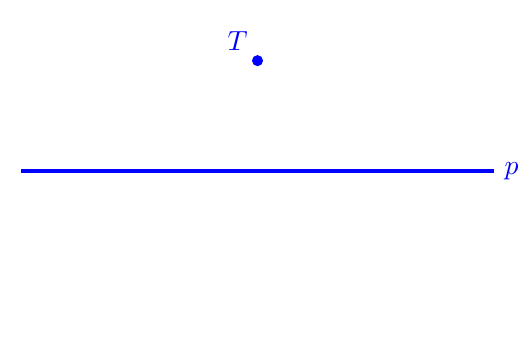
\includegraphics[width=50mm]{fig-1.png}}
            \only<2>{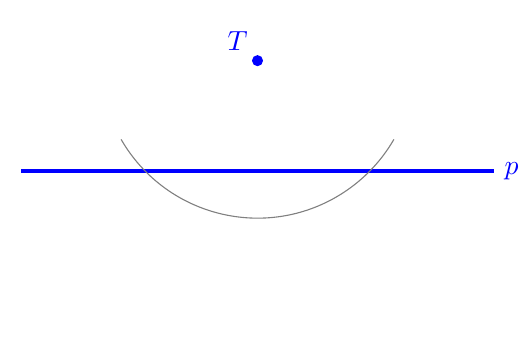
\includegraphics[width=50mm]{fig-2.png}}
            \only<3>{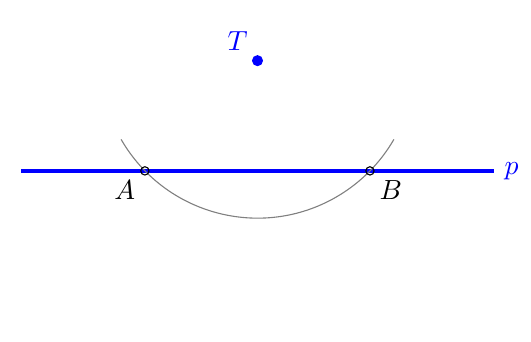
\includegraphics[width=50mm]{fig-3.png}}
            \only<4>{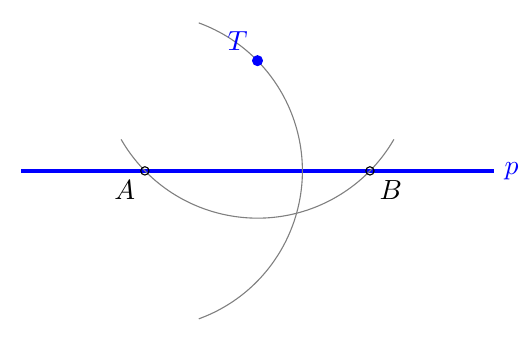
\includegraphics[width=50mm]{fig-4.png}}
            \only<5>{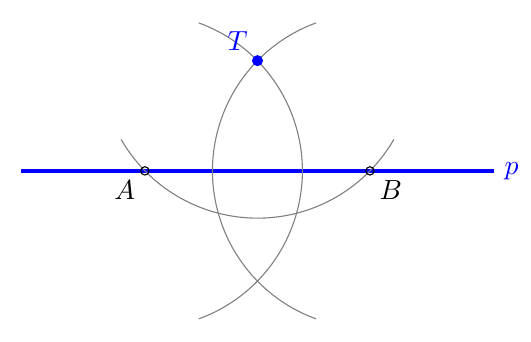
\includegraphics[width=50mm]{fig-5.png}}
            \only<6>{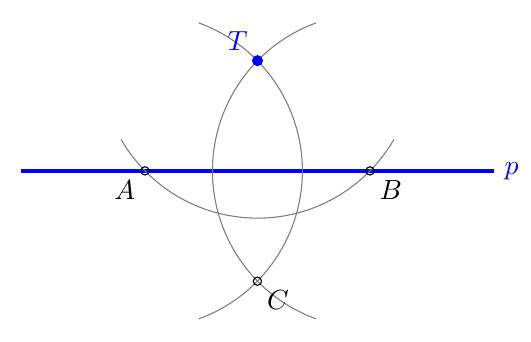
\includegraphics[width=50mm]{fig-6.png}}
            \only<7>{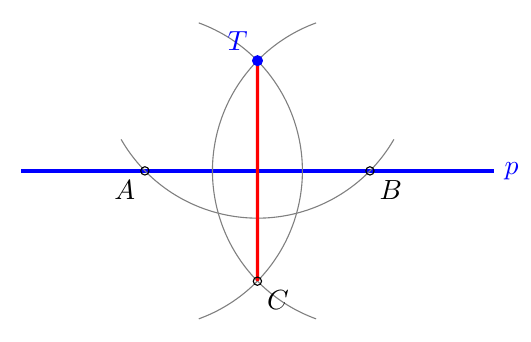
\includegraphics[width=50mm]{fig-7.png}}
        \end{column}
    \end{columns}
\end{frame}


\section{Paket \texttt{beamer} in tabele}
% Tabela po vrsticah: najprej samo glava, nato X, Y in Z.
\begin{frame}{Odkrivanje tabele po vrsticah}
    Včasih pride prav, da tabelo odkrivamo postopoma po vrsticah.
    \begin{center}
        \begin{tabular}{c|cccc}
            Oznaka & A & B & C & D \\ \hline
            \only<2->{X & 1 & 2 & 3 & 4 \\}
            \only<3->{Y & 3 & 4 & 5 & 6 \\}
            \only<4->{Z & 5 & 6 & 7 & 8 \\}
        \end{tabular}
    \end{center}
\end{frame}

% Tabela po stolpcih: vsaka kolona ima svoj predpis za prikaz.
\begin{frame}{Odkrivanje tabele po stolpcih}
    Tabelo lahko odkrivamo tudi po stolpcih, čeprav ni najlažje.
    \begin{center}
        \begin{tabular}{c|>{\onslide<2->}c<{\onslide} >{\onslide<3->}c<{\onslide} >{\onslide<4->}c<{\onslide} >{\onslide<5->}c<{\onslide}}
            Oznaka & A & B & C & D \\ \hline
            X & 1 & 2 & 3 & 4 \\
            Y & 3 & 4 & 5 & 6 \\
            Z & 5 & 6 & 7 & 8
        \end{tabular}
    \end{center}
\end{frame}


\section{Risanje s paketom TikZ}
% Koraki konstrukcije se razkrijejo na šestih podprosojnicah.
\begin{frame}{Konstrukcija pravokotnice}
    \centering
    \begin{tikzpicture}
        \coordinate (T) at (0,1.4);
        % Nevidne poti, ki omogočijo izračun presečišč na vseh podprosojnicah.
        \path[name path=p] (-3,0) -- (3,0);
        \path[name path=k] (T) ++(210:2) arc (210:330:2);
        \path[name intersections={of=p and k,by={A,B}}];
        \path[name path=m] (A) ++(-70:2) arc (-70:70:2);
        \path[name path=n] (B) ++(250:2) arc (250:110:2);
        \path[name intersections={of=m and n,by={C,Tprime}}];

        \draw[blue,very thick] (-3,0)--(3,0) node[right] {$p$};
        \draw<2->[gray] (T) ++(210:2) arc (210:330:2);
        \draw<3->[gray] (A) ++(-70:2) arc (-70:70:2);
        \draw<4->[gray] (B) ++(250:2) arc (250:110:2);
        \draw<6->[red,very thick] (T)--(C);

        \fill[blue] (T) circle (2pt) node[above left] {$T$};
        \only<2->{
            \draw (A) circle (1.5pt) node[below left] {$A$};
            \draw (B) circle (1.5pt) node[below right] {$B$};
        }
        \only<5->{\draw (C) circle (1.5pt) node[below right] {$C$};}
    \end{tikzpicture}
\end{frame}


\end{document}
